
% ----------------------------------------------------------------------
%  Set the document class
% ----------------------------------------------------------------------
\documentclass[11pt,a4paper,twoside]{article}

% ----------------------------------------------------------------------
% Define external packages, language, margins, fonts and new commands
% ----------------------------------------------------------------------
%\input{preamble} 
\usepackage[utf8]{inputenc}   % <<<<< Linux
\usepackage[english]{babel} % <<<<< English
\usepackage{notoccite}
\usepackage[skip=0.5\baselineskip]{caption}
\hyphenation{GTKWave}
\usepackage{listings}
\usepackage[all]{nowidow}

%blind text
\usepackage{lipsum}

\usepackage{graphicx}
\graphicspath{ {./} {../../figlib/} }
\def\FontLn{% 16 pt normal
  \usefont{T1}{phv}{m}{n}\fontsize{16pt}{16pt}\selectfont}
\def\FontLb{% 16 pt bold
  \usefont{T1}{phv}{b}{n}\fontsize{16pt}{16pt}\selectfont}
\def\FontMn{% 14 pt normal
  \usefont{T1}{phv}{m}{n}\fontsize{14pt}{14pt}\selectfont}
\def\FontMb{% 14 pt bold
  \usefont{T1}{phv}{b}{n}\fontsize{14pt}{14pt}\selectfont}
\def\FontSn{% 12 pt normal
  \usefont{T1}{phv}{m}{n}\fontsize{12pt}{12pt}\selectfont}

% Use Arial font as default
%
\renewcommand{\rmdefault}{phv}
\renewcommand{\sfdefault}{phv}
\usepackage{geometry}	
\geometry{verbose,tmargin=2.5cm,bmargin=2.5cm,lmargin=2.5cm,rmargin=2.5cm}

%\usepackage{setspace}
%\renewcommand{\baselinestretch}{1.5}

\usepackage[pdftex]{hyperref} % enhance documents that are to be
                              % output as HTML and PDF
\hypersetup{colorlinks,       % color text of links and anchors,
                              % eliminates borders around links
%            linkcolor=red,    % color for normal internal links
            linkcolor=black,  % color for normal internal links
            anchorcolor=black,% color for anchor text
%            citecolor=green,  % color for bibliographical citations
            citecolor=black,  % color for bibliographical citations
%            filecolor=magenta,% color for URLs which open local files
            filecolor=black,  % color for URLs which open local files
%            menucolor=red,    % color for Acrobat menu items
            menucolor=black,  % color for Acrobat menu items
%            pagecolor=red,    % color for links to other pages
            pagecolor=black,  % color for links to other pages
%            urlcolor=cyan,    % color for linked URLs
            urlcolor=black,   % color for linked URLs
	          bookmarks=true,         % create PDF bookmarks
	          bookmarksopen=false,    % don't expand bookmarks
	          bookmarksnumbered=true, % number bookmarks
	          pdftitle={report},
            pdfauthor={Andre C. Marta},
%            pdfsubject={Thesis Title},
%            pdfkeywords={Thesis Keywords},
            pdfstartview=FitV,
            pdfdisplaydoctitle=true}

\usepackage[numbers,sort&compress]{natbib} % <<<<< References in numbered list [1],[2],...
\usepackage{subcaption} 
\usepackage{mdframed}
\usepackage{placeins}
%\usepackage{setspace}

%%%%%%%%%%%%%%%%%%%%%%%%%%%%%%%%%%%%%%%%%%%%%%%%%%%%%%%%%%%%%%%%%%%%%%%%
%     Begin Document                                                   %
%%%%%%%%%%%%%%%%%%%%%%%%%%%%%%%%%%%%%%%%%%%%%%%%%%%%%%%%%%%%%%%%%%%%%%%%


\begin{document}

% Set plain page style (no headers, footer with centered page number)
\pagestyle{plain}

% Set roman numbering (i,ii,...) before the start of chapters
%\pagenumbering{roman}

% ----------------------------------------------------------------------
%  Cover page
% ----------------------------------------------------------------------

\thispagestyle {empty}

% IST Logo - Signature A
% parameters: bb=llx lly urx ury (bounding box), width=h_length, height=v_length, angle=angle, scale=factor, clip=true/false, draft=true/false. 
\includegraphics[bb=9.5cm 11cm 0cm 0cm,scale=0.29]{IST_A_CMYK_POS}

\begin{center}
%
% Figure (Image or plot)
\vspace{1.0cm}
% height = 50 mm
%\includegraphics[height=50mm]{Figures/Airbus_A350.jpg}

% Title, author and degree
\vspace{1cm}
{\FontLb Circuit Theory and Electronics Fundamentals} \\ % <<<<< EDIT TITLE
\vspace{1cm}
{\FontSn Integrated Master's in Aerospace Engineering, Técnico, University of Lisbon} \\ 
\vspace{1cm}
{\FontSn Laboratory 2 Report} \\ 
\vspace{1cm}
{\FontSn Francisco Alves 95787, Tomás Nunes 95855, Rodrigo Sequeira 96480} \\ 
\vspace{1cm}
{\FontSn April 5th, 2021} 
%
\end{center}



% ----------------------------------------------------------------------
% Dedication page (optional)
% ----------------------------------------------------------------------
%\input{dedication} 
%\cleardoublepage

% ----------------------------------------------------------------------
%  Acknowledgments (optional)
% ----------------------------------------------------------------------
%\input{acknowledgements}
%\cleardoublepage

% ----------------------------------------------------------------------
%  Abstract (both in English and Portuguese)
% ----------------------------------------------------------------------
%\input{resumo} 
%\cleardoublepage

%\input{abstract} 

% ----------------------------------------------------------------------
%  Table of contents, list of tables, list of figures and nomenclature
% ----------------------------------------------------------------------

% Table of contents
%
%\singlespacing
\tableofcontents

% List of tables
%\addcontentsline{toc}{section}{\listtablename}
%\listoftables
%\cleardoublepage 

% List of figures
%\addcontentsline{toc}{section}{\listfigurename}
%\listoffigures
%\cleardoublepage 

% Set arabic numbering (1,2,...) after preface
%
%\setcounter{page}{1}
%\pagenumbering{arabic}

% ----------------------------------------------------------------------
%  Body
% ----------------------------------------------------------------------
%\pagebreak
\section{Introduction}
\label{sec:introduction}

In this laboratory assignment, we are asked to create an Audio Amplififer Circuit, in which we are supposed to design the architecture of the Gain and Output stages of the circuit. The goal is to achieve the best ratio between the cost of the circuit and its quality in terms of the specifications asked (Merit Figure): the gain's frequency response and the input and output impedances. \par
To build the circuit, we used 7 resistors, 3 capacitors and 2 transistors (one PNP type and one NPN type). A representative image of the circuit can be seen in \ref{fig:t4}. \par
As stated, the circuit has 2 different stages (gain and output), where the first one amplifies the input signal and the last one increases the output current. The gain stage is characterized by a high gain but the output impedance is also high, whereas the output stage has a near 1 gain with a low output impedance.


In Section \ref{sec:analysis}, a theoretical analysis of the circuit using Octave is
presented. In Section \ref{sec:simulation}, the circuit is analysed by
simulation with Ngspice software and the results are compared to the theoretical results in Section \ref{sec:sbs}. Conclusions of this study can be found in
Section \ref{sec:conclusion}.

The components used have the following values:
\begin{table}[h]
\centering
\begin{small}
\caption{Values in SI units.}
\begin{tabular}{|c|c|}
\hline
$R_{in}$ & 100 \\
$R_1$ & 100000 \\
$R_2$ & 20000 \\
$R_c$ & 500 \\
$R_e$ & 100 \\
$R_{out}$ & 100 \\
$C_i$ & 0.001000 \\
$C_b$ & 0.005000 \\
$C_o$ & 0.001995 \\
\hline
\end{tabular}
\end{small}
\end{table}

\begin{figure}[htp] \centering
\includegraphics[width=0.8\linewidth]{t4.pdf}
\caption{Circuit in study.}
\label{fig:t4}
\end{figure}
\FloatBarrier



\section{Theoretical Analysis}
\label{sec:analysis}

In this section, the circuit shown in Figure \ref{fig:t4} is analysed 
theoretically.

For the gain stage, we assigned the values $R_S=100\Omega$, $V_T=25\times 10^3 V$, $\beta _{FN}=178.7 $, $V_{AFN}=69.7 V$, $R_{E1}=100 \Omega$, $R_{C1}=500 \Omega$, $R_{B1}=100000 \Omega$, $R_{B2}=20000 \Omega$, $V_{BEON}=0.7 V$, $V_{CC}=12 V$ and defined $R_{SB}$ as

\begin{equation*} \label{eq1}
R_{SB}=\frac{R_B\times R_S}{R_B+R_S}
\end{equation*}

$g_{m1}$ as

\begin{equation*} \label{eq2}
g_{m1}=I_{C1}/V_T
\end{equation*}

$r_{\pi 1}$ as

\begin{equation*} \label{eq3}
r_{\pi 1}=\frac{\beta _{FN}}{g_{m1}}
\end{equation*}

and $r_{o1}$ as

\begin{equation*} \label{eq4}
r_{o1}=\frac{V_{AFN}}{I_{C1}}
\end{equation*}

For the output stage, we assigned the values $\beta _{FP} = 227.3$, $V_{AFP} = 37.2 V$, $R_{E2} = 100 \Omega$, $V_{EBON} = 0.7 V$, $V_{I2} = V_{O1}$, $I_{E2} = \frac{V_{CC}-V_{EBON}-V_{I2}}{R_{E2}}$, $I_{C2} = \frac{\beta _{FP}}{(\beta _{FP}+1)I_{E2}}$,
$V_{O2} = V_{CC} - R_{E2}\times I_{E2}$ and defined $g_{m2}$ as

\begin{equation*} \label{eq7}
g_{m2} = \frac{I_{C2}}{V_T}
\end{equation*}

$g_{o2}$ as

\begin{equation*} \label{eq8}
g_{o2} = \frac{I_{C2}}{V_AFP}
\end{equation*}

$g_{\pi 2}$ as

\begin{equation*} \label{eq9}
g_{\pi 2} = \frac{g_{m2}}{\beta _{FP}}
\end{equation*}

and $g_{e2}$ as 

\begin{equation*} \label{eq10}
g_{e2} = \frac{1}{R_{E2}}
\end{equation*}

\subsection{Operating point}
In this analysis, the circuit used is the one presented in Figure \ref{fig:t4}.
The operating points were computed for both the gain and output stages to verify that the transistors had the acceptable voltages to be functioning. \par
The NPN transistor used in the gain stage had to obey $V_{CE}>V_{BEON}=0.7 V$. \par
The PNP transistor used in the output stage had to obey $V_{EC}=V_{O2}>V_{EBON}=0.7 V$. \par
In the following table, we present the operating point values.

\quad Gain stage:
Firstly, we have
\begin{equation*}
R_B=\frac{1}{\frac{1}{R_{B1}}+\frac{1}{R_{B2}}}
\end{equation*}

\begin{equation*}
V_{EQ}=\frac{R_{B2}}{R_{B1}+R_{B2}}V_{CC}
\end{equation*}

\begin{equation*}
I_{B1}=\frac{V_{EQ}-V_{BEON}}{R_B+(1+\beta _{FN})*R_{E1}}
\end{equation*}

\begin{equation*}
I_{C1}=\beta _{FN}\times I_{B1}
\end{equation*}

\begin{equation*}
I_{E1}=(1+\beta _{FN})I_{B1}
\end{equation*}

\begin{equation*}
V_{E1}=R_{E1}\times I_{E1}
\end{equation*}

\begin{equation*}
V_{O1}=V_{CC}-R_{C1}\times I_{C1}
\end{equation*}

\begin{equation*}
V_{CE}=V_{O1}-V_{E1}
\end{equation*}

\quad Output stage:

\begin{equation*}
V_{I2}=V_{O1}
\end{equation*}

\begin{equation*}
I_{E2}=\frac{V_{CC}-V_{EBON}-V_{I2}}{R_{E2}}
\end{equation*}

\begin{equation*}
I_{C2}=\frac{\beta _{FP}}{\beta _{FP}+1} \times I_{E2}
\end{equation*}

\begin{equation*}
V_{O2}=V_{CC}-R_{E2} \times I_{E2}
\end{equation*}

\begin{table}[h]
  \centering
  \begin{tabular}{|l|r|}
    \hline    
    {\bf Name} & {\bf Value [V]} \\ \hline
    $V_{CE}$ & 7.972014\\ \hline
$V_{BE}$ & 0.7000000\\ \hline
$V_{O1}$ & 8.646473\\ \hline
$V_{EC}$ & 9.346473\\ \hline
$V_{EB}$ & 0.7000000\\ \hline
$V_{O2}$ & 9.346473\\ \hline

  \end{tabular}
  \caption{Operating point}
  \label{tab:OP}
\end{table}

Note that both transistors are working in the Forward Active Region.


\subsection{Gain, input and output impedances}

To obtain the following values we need to analyse the incremental circuit version of the original circuit.  \par

\quad Gain stage:
We can write the following equations: 
-To compute the gain stage's gain,

\begin{equation} \label{eq5}
R_{E1}=0 , AV_1 = \frac{R_{SB}}{R_S} \times \frac{R_{C1}(R_{E1}-g_{m1}\times r_{\pi 1}\times r_{o1})}{(r_{o1}+R_{C1}+R_{E1})\times(R_{SB}+r_{\pi 1}+R_{E1})+g_{m1}*R_{E1}*r_{o1}*r_{\pi 1} - R_{E1}^2)}
\end{equation}

-To compute the gain stage's input impedance
\begin{equation} \label{eq6}
R_{E1}=0 , Z_{I1} = \frac{1}{\frac{1}{R_B}+\frac{1}{\frac{(r_{o1}+R_{C1}+R_{E1})\times(r_{\pi 1}+R_{E1})+g_{m1}\times R_{E1}\times r_{o1}\times r_{\pi 1} - R_{E1}^2}{r_{o1}+R_{C1}+R_{E1}}}}
\end{equation}

-To compute the gain stage's output impedance
\begin{equation}\label{eqesq}
Z_{O1} = \frac{1}{\frac{1}{r_{o1}}+\frac{1}{R_{C1}}}
\end{equation}

\quad Output stage:

We can write the following equations:

-To compute the output stage's gain, 
\begin{equation} \label{eq11}
AV_2 = \frac{g_{m2}}{g_{m2}+g_{\pi 2}+g_{o2}+g_{e2}}
\end{equation}

-To compute the output stage's input impedance,
\begin{equation} \label{eq12}
Z_{I2} = \frac{g_{m2}+g_{\pi 2}+g_{o2}+g_{e2}}{g_{\pi 2}(g_{\pi 2}+g_{o2}+g_{e2})}
\end{equation}

-To compute the output stage's output impedance,
\begin{equation} \label{eq13}
Z_{O2} = \frac{1}{g_{m2}+g_{\pi 2}+g_{o2}+g_{e2}}
\end{equation}

The following table presents the values for the gain, input impedance and output impedance of both stages.

\begin{table}[h]
  \centering
  \begin{tabular}{|l|r|}
    \hline    
    {\bf Name} & {\bf Value [$\Omega$]} \\ \hline
    $Z_{I1}$ & 640.4922\\ \hline
$Z_{O1}$ & 477.0475\\ \hline
$AV_{1}$ & 110.6998\\ \hline
$Z_{I2}$ & 15013.86\\ \hline
$Z_{O2}$ & 0.9327305\\ \hline
$AV_{2}$ & 0.9856738\\ \hline

  \end{tabular}
  \caption{Gain, input impedance and output impedance}
  \label{tab:OP}
\end{table}
\FloatBarrier

\quad Total:

In order to make a comparison with the simulation's gain, and input and output impedances, we computed the theoretical values for these variables.

\begin{equation} \label{eq13}
g_B = \frac{1}{\frac{1}{g_{\pi 2}}+Z_{O1}}
\end{equation}

\begin{equation} \label{eq13}
AV = AV_1\frac{\frac{g_B+g_{m2}}{g_{\pi 2}\times g_B}}{g_B+g_{e2}+g_{o2}+\frac{g_{m2}}{g_{\pi 2}}\times g_B}
\end{equation}

\begin{equation} \label{eq13}
Z_I=Z_{I1}
\end{equation}

\begin{equation} \label{eq13}
Z_O=\frac{1}{g_{o2}+\frac{g_{m2}}{g_\pi 2}\times g_B+g_{e2}+g_B}
\end{equation}

\begin{table}[h]
  \centering
  \begin{tabular}{|l|r|}
    \hline    
    {\bf Name} & {\bf Value [$\Omega$]} \\ \hline
    $Z_{I}$ & 640.4922\\ \hline
$Z_{O}$ & 2.9364\\ \hline
$AV$ & 107.21838\\ \hline

  \end{tabular}
  \caption{Gain, input impedance and output impedance}
  \label{tab:OP}
\end{table}
\FloatBarrier

\subsection{Frequency response}
In order to obtain the Merit Figure of our circuit, we tried to compute the theoretical value of the bandwidth. However, we were only able to obtain the value of the lower cut off frequency as seen in \ref{fig:gain}, so we used Ngspice's value for the upper cut off frequency. This is due to the fact that for this frequency we need to take parasite capacitors into account which would lead to complex calculations.

\begin{table}[h]
  \centering
  \begin{tabular}{|l|r|}
    \hline    
    {\bf Name} & {\bf Value [Hz]} \\ \hline
    $uco$ & 3106930.0\\ \hline
$lco$ & 11.75169\\ \hline
$bandwith$ & 3106918.25\\ \hline

  \end{tabular}
  \caption{Bandwith}
  \label{tab:OP}
\end{table}
\FloatBarrier

\begin{figure}[h] \centering
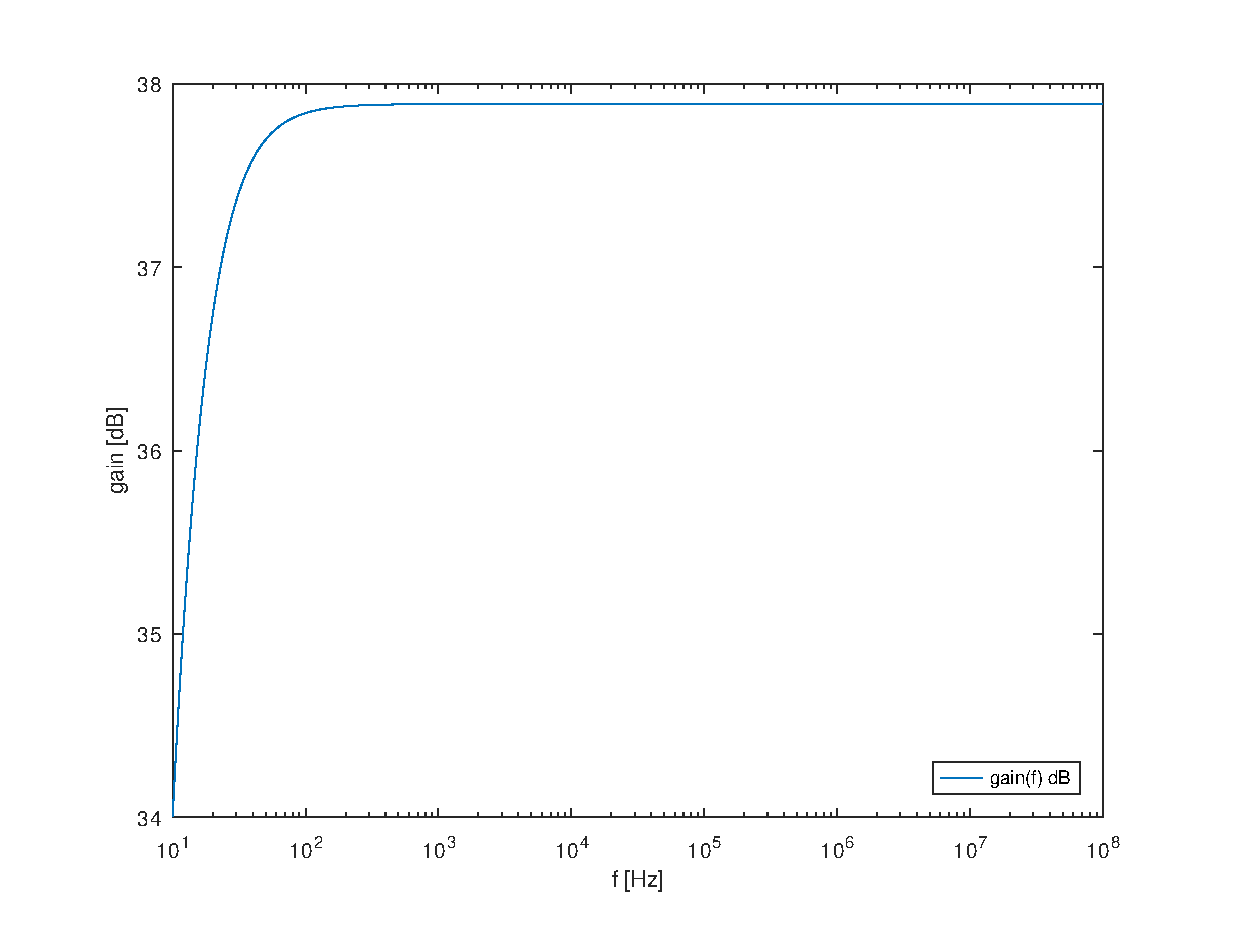
\includegraphics[width=0.6\linewidth]{gain_db_teo.eps}
\caption{Output voltage gain in order to frequency}
\label{fig:gain}
\end{figure}
\FloatBarrier

Here we present the merit figure of our circuit.

\begin{table}[h]
  \centering
  \begin{tabular}{|l|r|}
    \hline    
    {\bf Name} & {\bf Value [Mu]} \\ \hline
    $cost$ & 8116.008\\ \hline
$merit$ & 3492.661\\ \hline

  \end{tabular}
  \caption{Merit figure}
  \label{tab:OP}
\end{table}
\FloatBarrier


\section{Simulation Analysis}
\label{sec:simulation}

\subsection{Operating point for t$<$0}

Table \ref{tab:op_1} shows the simulated operating point results for the circuit analysis when t$<$0. Once again, current flows are the ones referred in section \ref{sec:analysis} and node 0 is considered to have 0V potential. \par
 A new voltage source $V_{aux}$ with voltage 0V (so it doesn't affect the circuit) was added to the circuit between components $R_6$ and $R_7$ so that Ngspice could simulate and calculate the current value in that branch. This current is needed since the voltage source $v_d$ depends on its value and as expected, this current's value is the same as the one that flows through $R_6$ and $R_7$. Adding a new voltage source led to the creation of node 8 between $R_6$ and $V_{aux}$. Also, as predicted, voltage $V_8$ is the same as voltage $V_6$ since the voltage in $V_{aux}$ is 0V.

\begin{table}[h]
  \centering
  \begin{tabular}{|l|r|}
    \hline    
    {\bf Name} & {\bf Value [A or V]} \\ \hline
    \input{../sim/op1_tab}
  \end{tabular}
  \caption{Operating point for t$<$0. A variable proceeded by [i] is of type {\em current}
    and expressed in Ampere; other variables are of type {\it voltage} and expressed in
    Volt.}
  \label{tab:op_1}
\end{table}
\FloatBarrier

\subsection{Operating point for $v_S$(0) = 0}

Table \ref{tab:op_2} shows the simulated operating point values for the circuit when t=0 and $v_S$(0) = 0V. The reason why this step is needed is the same as the one referred in \ref{sec:2.2}. Also, in order to perform the transient analysis, we replaced the capacitor with an independent voltage source from node 5 to 7 with value $V_x$. 

\begin{table}[h]
  \centering
  \begin{tabular}{|l|r|}
    \hline    
    {\bf Name} & {\bf Value [A or V or $\Omega$]} \\ \hline
    \input{../sim/op2_tab}
  \end{tabular}
  \caption{Operating point for $v_S$(0) = 0. A variable proceeded by [i], and $I_x$ is of type {\em current}
    and expressed in Ampere; other variables are of type {\it voltage} and expressed in
    Volt, except $R_e$$_q$ that is in Ohm.}
  \label{tab:op_2}
\end{table}
\FloatBarrier

\subsection{Natural response}

In this step, the natural response of the circuit with a given boundary condition is simulated using Ngspice's transient analysis function. The boundary condition is $V_5$ and $V_7$ obtained in the previous subsection when t=0. After comparing the results we concluded that the values obtained in Ngspice matched the ones from Octave, so we used the Octave values directly in Ngspice. The plot for t$\in$[0;20]ms can be seen in \ref{fig:v5_ng}. 

\begin{figure}[h] \centering
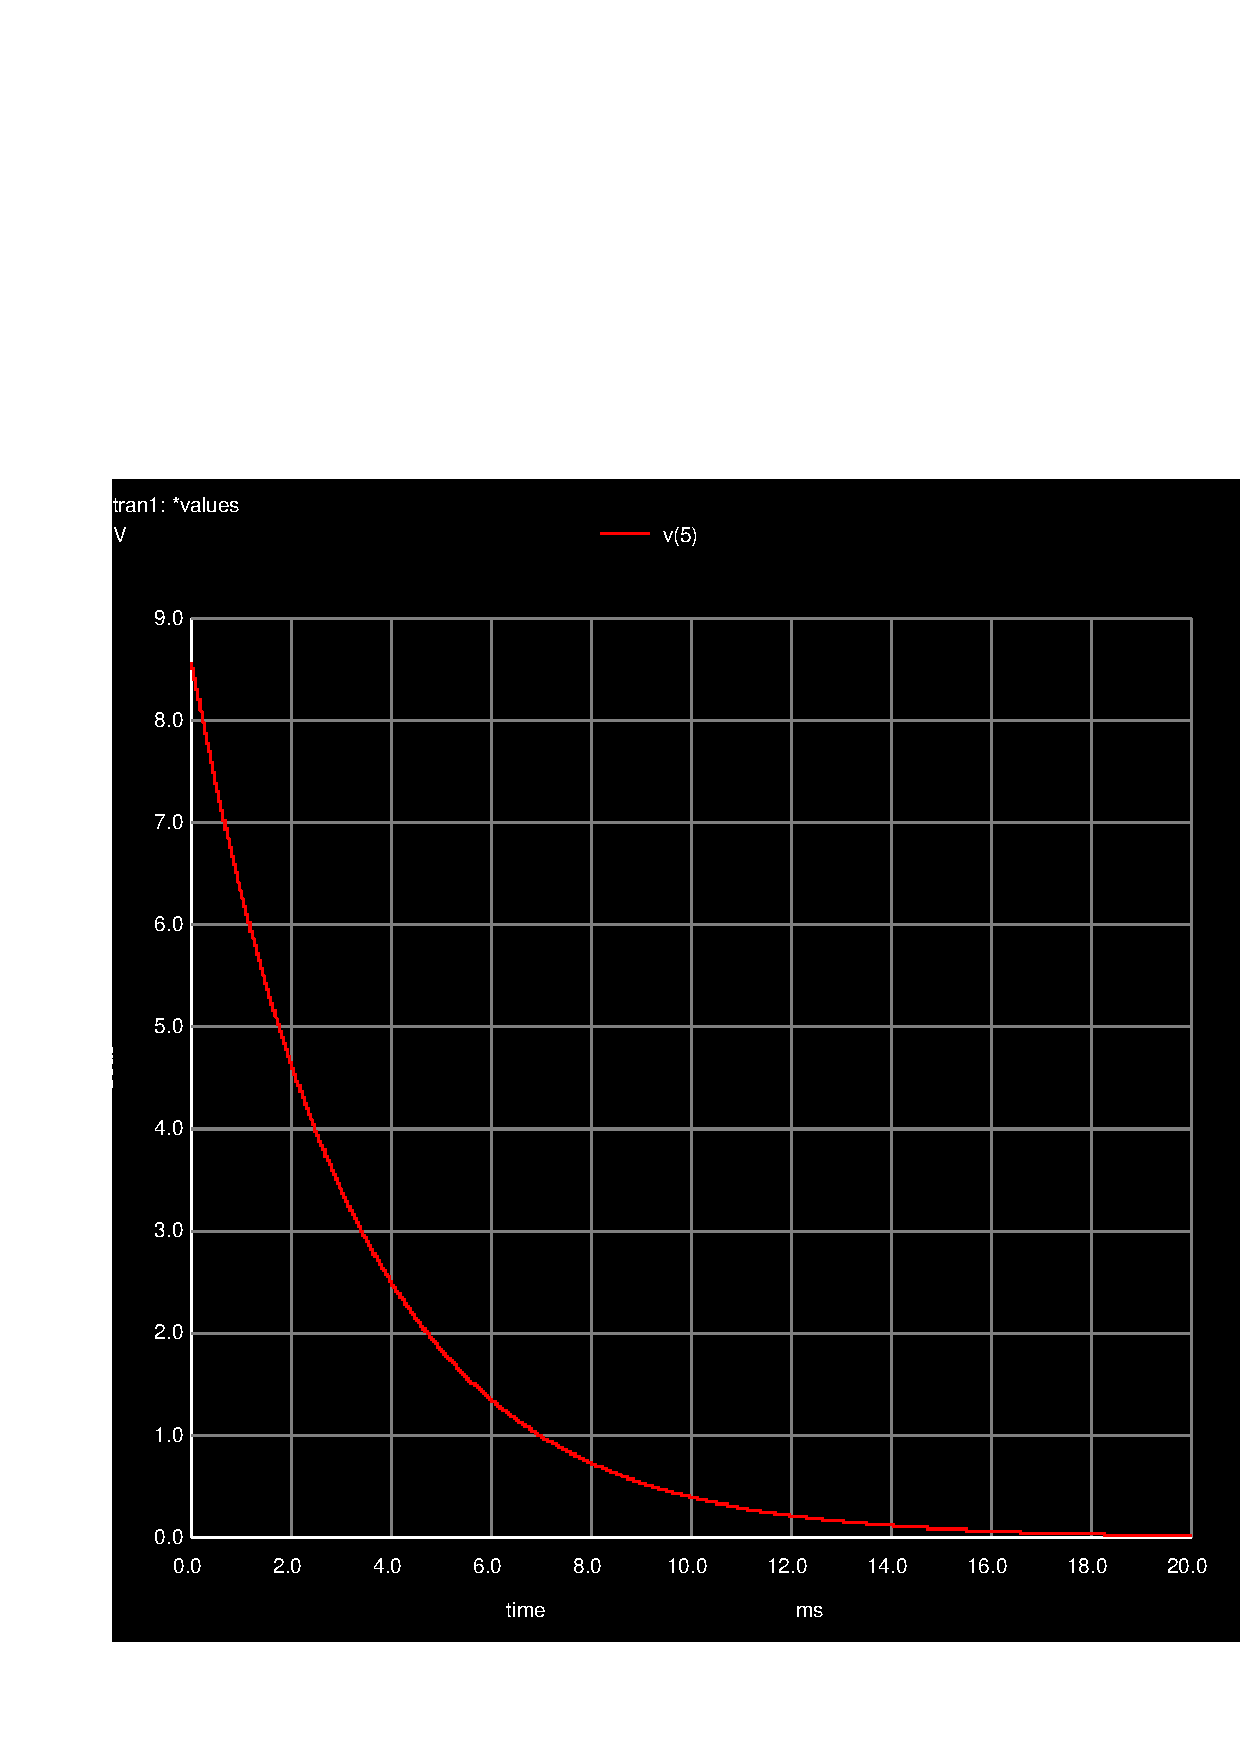
\includegraphics[width=0.6\linewidth]{transv5n.pdf}
\caption{Natural solution for $v_5$}
\label{fig:v5_ng}
\end{figure}
\FloatBarrier

\subsection{Natural and forced responses for f = 1kHz and given $v_S$(t)}

The plot for $v_S$(t) and the circuit's response can be seen in \ref{fig:transv5vs.pdf}.

\begin{figure}[h] \centering
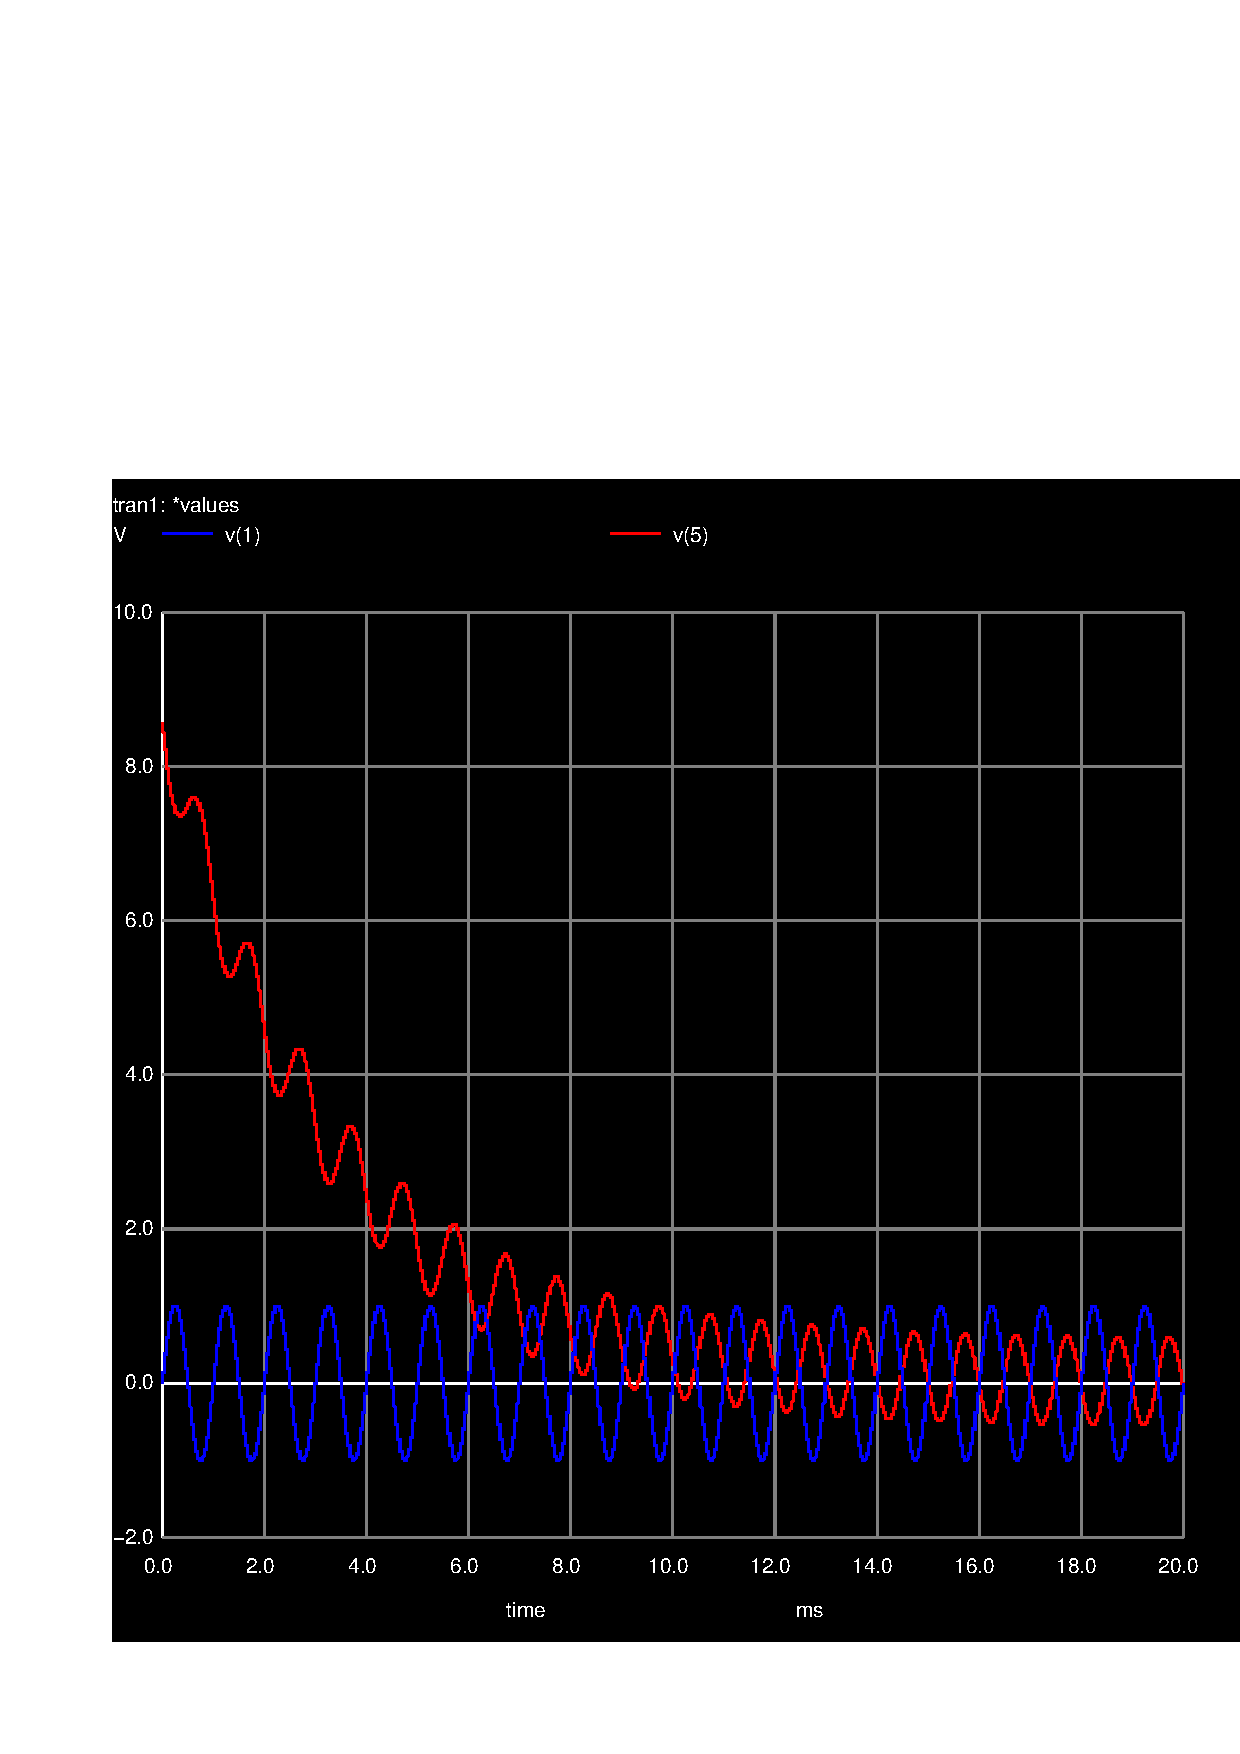
\includegraphics[width=0.6\linewidth]{transv5vs.pdf}
\caption{Stimulus (blue) and response (red) on node 5}
\label{fig:transv5vs.pdf}
\end{figure}
\FloatBarrier


\subsection{Frequency response}

For f$\in$[0.1Hz;1MHz] the frequency response in node 5 is simulated. The functions $v_S$(f) and $v_5$(f) are plotted in a logarithmic scale (dB) in \ref{fig:db_v5_v1.pdf}, and the phases can be seen in degrees in \ref{fig:phase.pdf}. The differences between these functions and the reasons why they have distinct behaviors are stated in \ref{sec:frequency}.
%EXPLICAR

\begin{figure}[h] \centering
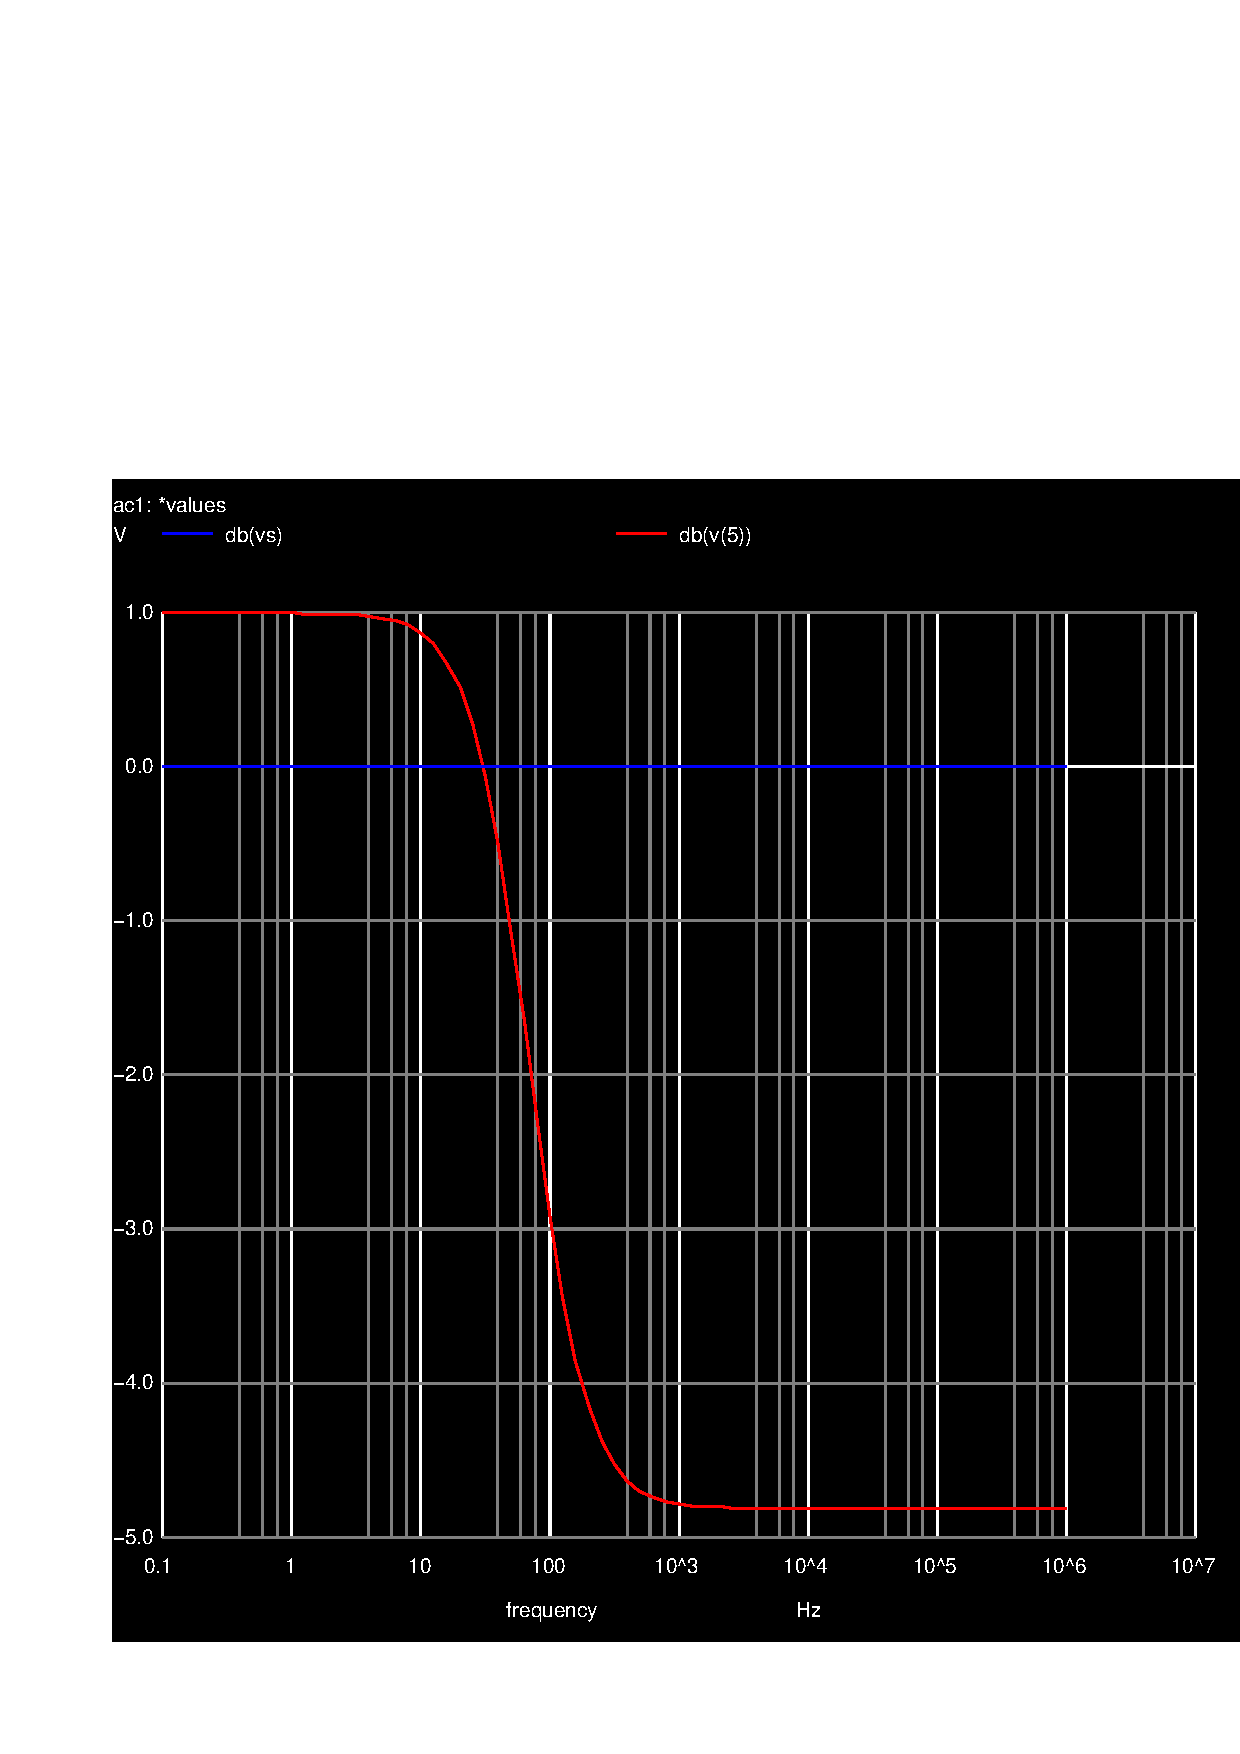
\includegraphics[width=0.6\linewidth]{db_v5_v1.pdf}
\caption{$v_S$(f), in blue, $v_5$(f), in red, and $v_C$(f), in yellow}
\label{fig:db_v5_v1.pdf}
\end{figure}
\FloatBarrier

\begin{figure}[h] \centering
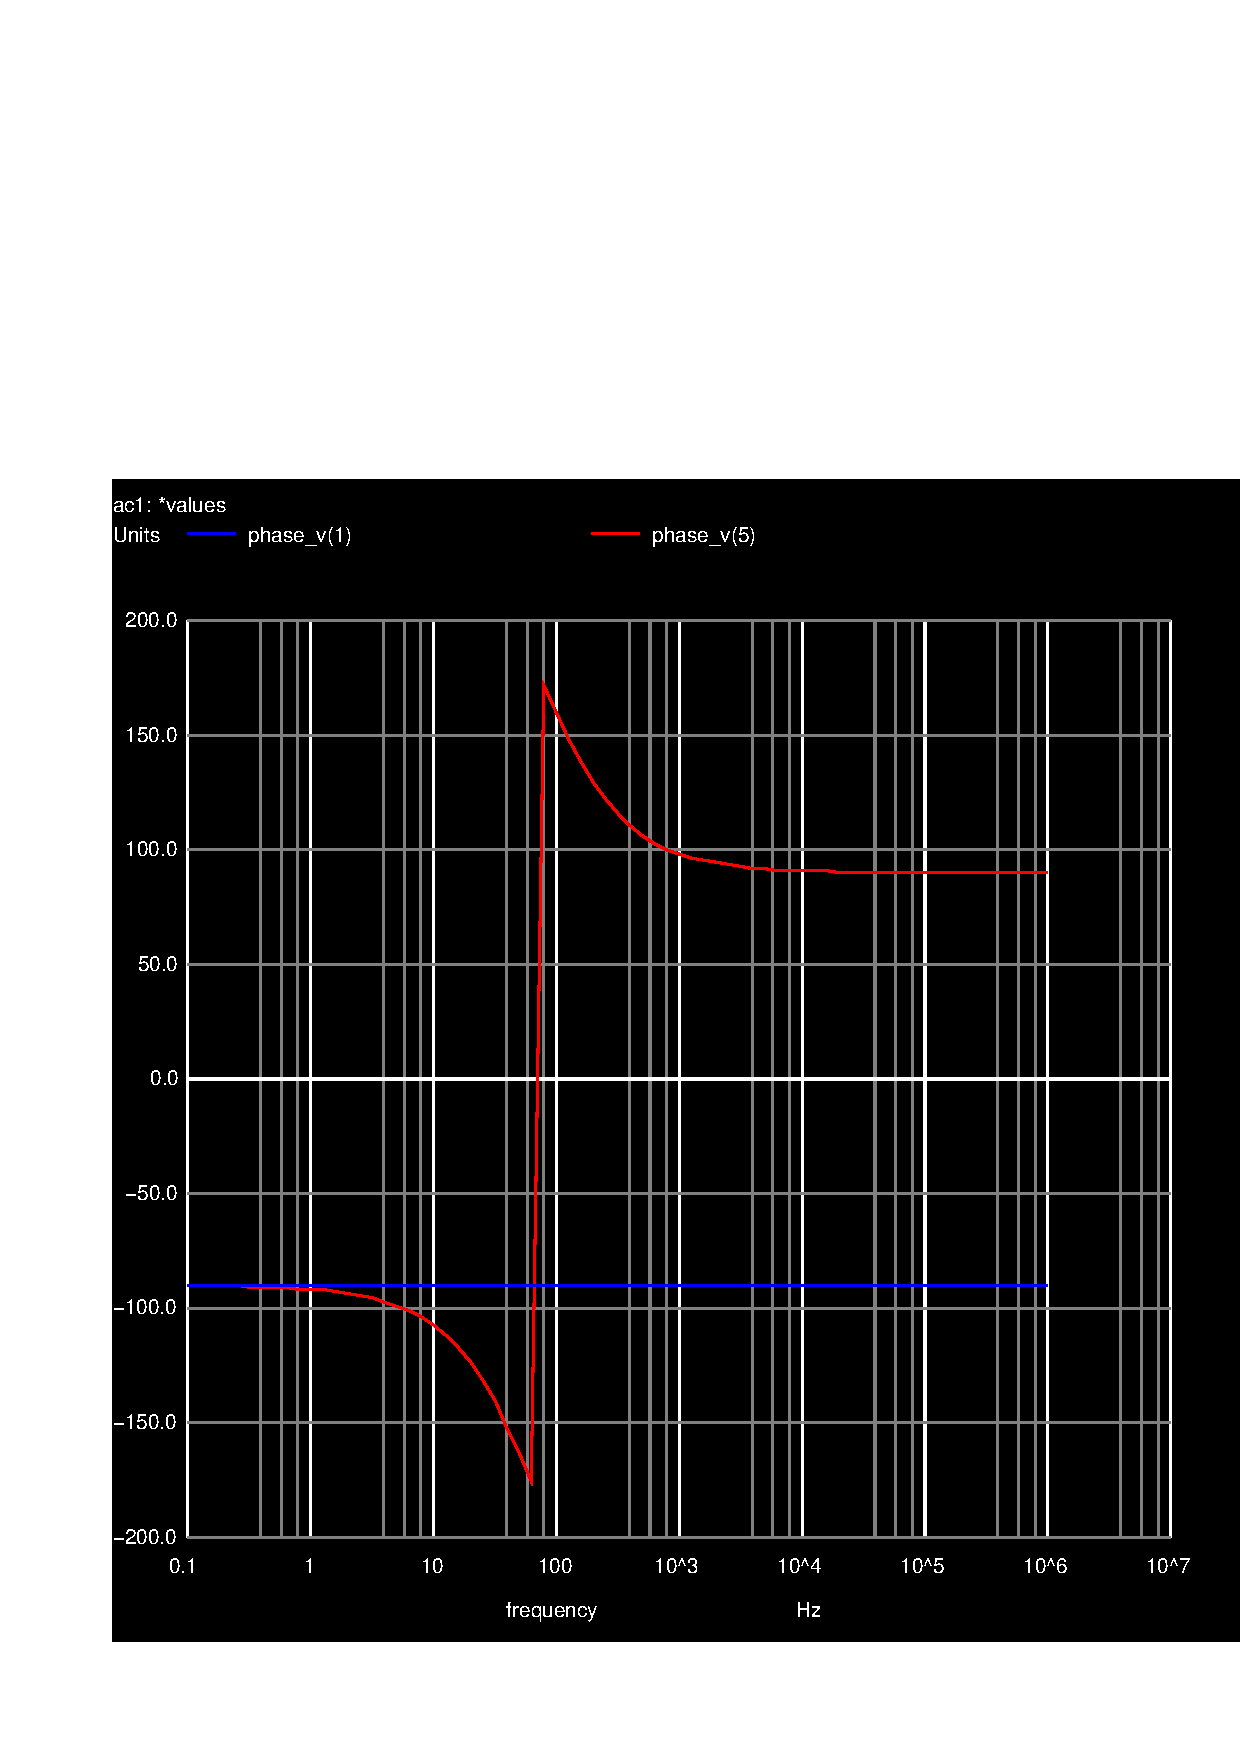
\includegraphics[width=0.6\linewidth]{phase.pdf}
\caption{Phase of $v_S$(f), in blue, $v_5$(f), in red, and $v_C$(f), in yellow}
\label{fig:phase.pdf}
\end{figure}
\FloatBarrier


\section{Conclusion}
\label{sec:conclusion}

In this laboratory assignment the objective of analysing an RC circuit has been
achieved. Static, time and frequency analyses have been performed both
theoretically using the Octave maths tool and by circuit simulation using the
Ngspice tool. The simulation results matched the theoretical results
precisely. The reason for this perfect match is the fact that this is a
straightforward circuit containing only linear components, so the theoretical
and simulation models cannot differ. For more complex components, the
theoretical and simulation models could differ but this is not the case in this
work.

%\lipsum[1-1]

%\cleardoublepage

% ----------------------------------------------------------------------
%  Bibliography
% ----------------------------------------------------------------------
%\addcontentsline{toc}{section}{\bibname}
%\bibliographystyle{abbrvunsrtnat} % <<<<< SELECT IF USING REFERENCES BY NUMBER (CITATION ORDER)
%\bibliography{../../../BIBfile.bib}

% ----------------------------------------------------------------------
\end{document}
% ----------------------------------------------------------------------

